% ----------------------------------------------------------------------------
% Copyright (c) 2016 by Burkhardt Renz. All rights reserved.
% Die Vorlage für eine Abschlussarbeit in der Informatik am Fachbereich
% MNI der THM ist lizenziert unter einer Creative Commons
% Namensnennung-Nicht kommerziell 4.0 International Lizenz.
%
% Id:$
% ----------------------------------------------------------------------------

\chapter{Design}
\label{chapter:Design}
In diesem Kapitel werden die in \cref{chapter:Problembeschreibung} beschriebenen Problemstellung bearbeitet. Anfänglich werden Designziele definiert, die den Rahmen für die Konzipierung bilden. In \cref{section:Datenmodell} wird ein Datenmodell vorgestellt, welches sich an Standards von bereits existierenden Tracingmodellen orientiert. \cref{section:Verarbeitungsmodell} präsentiert ein Konzept zur verarbeitung der erhobenen Tracingdaten. Der \cref{section:Visualisierung} beschäftigt sich mit der Darstellung der Tracingdaten zur Informationsgewinnen durch den Anwender der Bibliothek. Somit wird ein Konzept für dieTracinginfrastruktur zur Erhebung, Verarbeitung und Visualisierung von Tracingdaten vorgestellt.

\section{Designziele}
\label{section:Designziele}

Aus den in \cref{section:Anforderungsanalyse} beschriebenen Anforderungen folgern Designziele, die an das Design gestellt werden. Die von Google erstellte Fachpublikation \emph{Dapper, a Large-Scale Distributed Systems Tracing Infrastrcture} dient vielen Tracingsystemen als konzeptionelle Grundlage. In der Puplikation werden Designziele aufgeführt, die neue Tracingsysteme bewerten sollten. Es werden Designziele bewertet, die von Dapper genannt werden. Ausserdem sind zusätzliche Designziele aufgezeigt, die aus den Anforderungen des verteilten rendering Systems hervorkommen. Diese Designziele umfassen die (\lowroman{1}) \textbf{Verarbeitungskosten}, die (\lowroman{2}) \textbf{Benutzbarkeit}, die (\lowroman{3}) \textbf{Portabilität} und die (\lowroman{4}) \textbf{Datenverfügbarkeit}. Ausserdem werden Nicht-Ziele definiert. Zu diesen gehören die (\lowroman{5}) \textbf{Anwendungs-Level Transparenz} und die (\lowroman{6}) \textbf{Skalierbarkeit}.

\subsection{Ziele}
\label{subsection:Ziele}
\textbf{Verarbeitungskosten} \space\space\space Ein für die Performance der Anwendung kritisches Designziel, in der Tracing eingeführt werden soll, stellt der \textbf{Overhead} dar. Der Overhead, der durch die Instrumentalisierung entsteht, soll möglichst gering sein. So kann etwa in spezialisierten hochperfomanten Services kleinster, durch Instrumentalisierung entstehender Mehraufwand, deutlich merkbar sein.\footpartcite{Shanbhag2010}. 

\textbf{Benutzbarkeit} \space\space\space Die Benutzbarkeit des Tracingsystems soll durch die Verwendung von Standards gewährleistet sein. Die von \emph{Opentracing} veröffentlichte \gls{apiLabel} soll der Instrumentalisierungsbibliothek eine vertraute und bewährte Anwendererfahrung liefern. 

\textbf{Portabilität} \space\space\space Ein weiteres Designziel soll eine gegebene \textbf{Portabilität} sein. Die Umgebung für die das Tracingsystem entwicklet wird, ist eine Mischung aus Platformabhängigen und Platformunabhängigen Komponenten. Durch den verminderten Mehraufwand der bei platformunabhängigen Komponeten entsteht, wird eine verbesserte Nutzerfreundlichkeit gewährleistet. Vorallem bei der Integration in bestehende Systeme wird dies bemerkbar, da Bauprozesse von Projekten platformabhängig sind. Der platformabhängige Bauprozess soll im Falle des verteilten rendering System nicht beeinflusst werden. Die 

\textbf{Datenverfügbarkeit} \space\space\space Die Datenverfügbarkeit soll zeitnah stattfinden. Die von der Tracinginfrastruktur generierten Tracingdaten sollen zur Laufzeit darsgestellt werden. 

\subsection{Nicht-Ziele}
\label{subsection:Nicht-Ziele}

Die von Dapper genannten Designziele der \emph{Anwendungs-Level Transparenz} und der \emph{Skalierbarkeit} spielen für das verteilte rendering System eine untergeordnete Rolle. Diese Bewertung hat ihren Ursprung aus einer interpretierten Form eines Sprichworts. 

\begin{quote}
	Du bist nicht Google, also versuch auch nicht Google zu sein
\end{quote}

Dapper ist für eine Infrastruktur konzipiert, die globalen  Maßstäben entspricht. Das verteilte rendering System entspricht nicht diesen Maßstäben, somit soll auch die Tracinginfrastruktur diese nicht erfüllen müssen. Die beiden Deisgnziele von Dapper werden als Nicht-Ziele für das verteilte rendering System bewertet.

\textbf{Anwendungs-Level Transparenz}\space\space\space Instrumentalisierung erfordert eingreifen in Anwendungsquellcode. Dapper löst dies durch Ausnutzung von Bibliotheken. Diese werden Instrumentalisiert und in der Anwendungslogik verwendet. Somit ist die Tracinginfrastruktur für den Anwendungsentwickler nicht wahrnehmbar. Die Instrumentalisierung des verteilten rendering Systems soll an semantisch relevanten Bereichen stattfinden und flexibel sein. Dies gelingt durch direktes modifizieren der Anwendungslogik. Der Anwendungsentwickler muss sich dementsprechend selbst um die Instrumentalisierung kümmern. 

\textbf{Skalierbarkeit} \space\space\space Das verteilte rendering System ist, in seiner derzeiten Form, statisch. Das bedeutet, dass eine Skalierbarkeit keine zentrale Rolle in dem Design der Tracinginfrastruktur darstellt. Die Skalierbarkeit soll allerdings bewertet werden. 

\section{Datenmodell}
\label{section:Datenmodell}
\subsection{Eventmodell}
\label{subsection:Eventmodell}
\subsection{Eventgraph}
\label{subsection:Eventgraph}
\section{Verarbeitungsmodell}
\label{section:Verarbeitungsmodell}
\subsection{Agenten}
\label{subsection:Agenten}
\subsection{Collectoren}
\label{subsection:Collectoren}

\section{Visualisierung}
\label{section:Visualisierung}

\subsection{Tracegraph}
\subsection{Dreidimensionale Flammengraphen}
\begin{figure}[!ht]
	\centering
	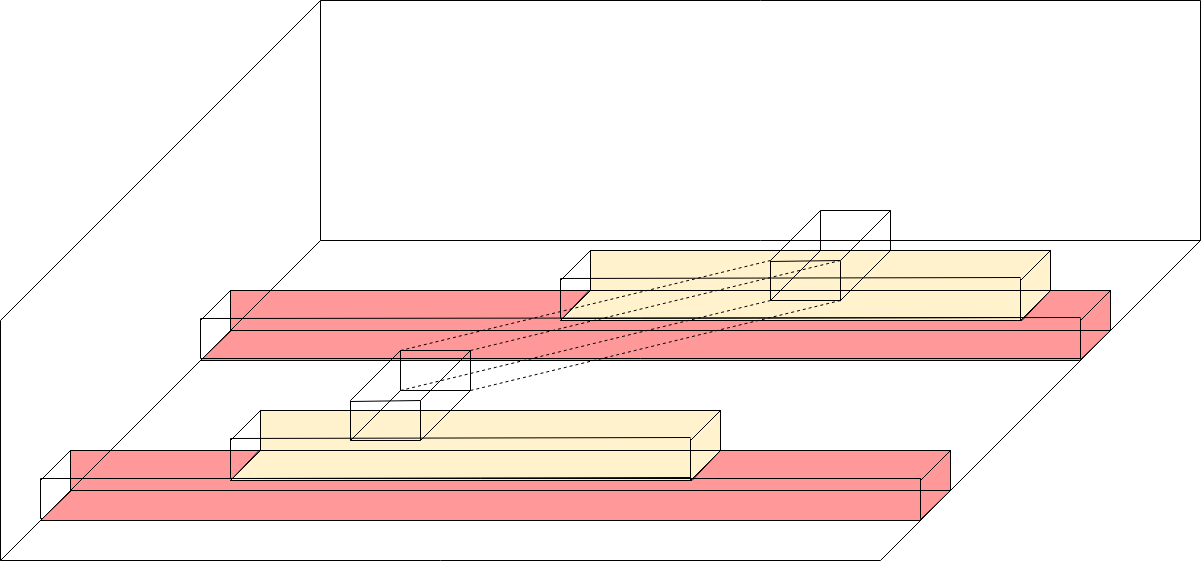
\includegraphics[scale=0.3]{img/Problembeschreibung/flamegraph_3D.png}
	\caption[3D Flammengraph]{Skizzierung eines dreidimensionalen Flammengraphs mit Nachrichtenaustausch}
	\label{fig:flamegraph_3D}
\end{figure}

% ----------------------------------------------------------------------------
